%%%%%%%%%%%%%%%%%%%%%%%%%%%%%%%%%%%%
%                                  %
% Titre  : p_i.tex                 %
% Sujet  : Manuel de l'utilisateur %
%          du projet 'PT-Scotch'   %
%          Introductions           %
% Auteur : Francois Pellegrini     %
%                                  %
%%%%%%%%%%%%%%%%%%%%%%%%%%%%%%%%%%%%

\section{Introduction}

\subsection{Static mapping}

The efficient execution of a parallel program on a parallel machine
requires that the communicating processes of the program be assigned
to the processors of the machine so as to minimize its overall running
time.
When processes have a limited duration and their logical dependencies
are accounted for, this optimization problem is referred to as
scheduling.
When processes are assumed to coexist simultaneously for the entire
duration of the program, it is referred to as mapping. It
amounts to balancing the computational weight of the processes among the
processors of the machine, while reducing the cost of communication by
keeping intensively inter-communicating processes on nearby
processors.

In most cases, the underlying computational structure of the parallel
programs to map can be conveniently modeled as a graph in which
vertices correspond to processes that handle distributed pieces of
data, and edges reflect data dependencies. The mapping problem can
then be addressed by assigning processor labels to the vertices of the
graph, so that all processes assigned to some processor are loaded and
run on it.
In a SPMD context, this is equivalent to the distribution
across processors of the data structures of parallel programs; in this
case, all pieces of data assigned to some processor are handled by a
single process located on this processor.

A mapping is called static if it is computed prior to the
execution of the program. Static mapping is NP-complete in the general
case~\cite{gajo79}. Therefore, many studies have been carried out in
order to find sub-optimal solutions in reasonable time, including
the development of specific algorithms for common topologies such
as the hypercube~\cite{errasa90,hamm92}.
When the target machine is assumed to have a communication network in
the shape of a complete graph, the static mapping problem turns into
the partitioning problem, which has also been intensely
studied~\cite{basi94,hele93a,kaku95a,kaku95c,posili90}.
However, when mapping onto parallel machines the communication network
of which is not a bus, not accounting for the topology of the target
machine usually leads to worse running times, because simple cut
minimization can induce more expensive long-distance
communication~\cite{hamm92,wacrevjo95}; the static mapping problem is
gaining popularity as most of the newer massively parallel machines
have a strongly NUMA architecture

\subsection{Sparse matrix ordering}

Many scientific and engineering problems can be modeled by sparse
linear systems, which are solved either by iterative or direct
methods.  To achieve efficiency with direct methods, one must minimize
the fill-in induced by factorization. This fill-in is a direct
consequence of the order in which the unknowns of the linear system
are numbered, and its effects are critical both in terms of memory and
of computation costs.
\\

Because there always exist large problem graphs which cannot fit in
the memory of sequential computers and cost too much to partition,
it is necessary to resort to parallel graph ordering tools.
\ptscotch\ provides such features.

\subsection{Contents of this document}

This document describes the capabilities and operations of \ptscotch,
a software package devoted to parallel static mapping and sparse
matrix block ordering.
It is the parallel extension of \scotch, a sequential software package
devoted to static mapping, graph and mesh partitioning, and sparse
matrix block ordering. While both packages share a significant amount
of code, because \ptscotch\ transfers control to the sequential
routines of the \libscotch\ library when the subgraphs on which it
operates are located on a single processor, the two sets of routines
have a distinct user's manual. Readers interested in the sequential
features of \scotch\ should refer to the {\it\scotch\ User's
Guide}~\scotchcitesuser.

The rest of this manual is organized as follows.
Section~\ref{sec-project} presents the goals of the \scotch\ project, and
section~\ref{sec-algo} outlines the most important aspects of the
parallel partitioning and ordering algorithms that it implements.
Section~\ref{sec-file} defines the formats of the files used in \ptscotch,
section~\ref{sec-prog} describes the programs of the
\ptscotch\ distribution, and section~\ref{sec-lib} defines the interface
and operations of the parallel routines of the \libscotch\ library.
Section~\ref{sec-install} explains how to obtain and install the
\scotch\ distribution.
Finally, some practical examples are given in
section~\ref{sec-examples}.
%, and instructions on how to implement new methods in the
%\libscotch\ library are provided in section~\ref{sec-coding}.

\section{The \scotch\ project}
\label{sec-project}

\subsection{Description}

\scotch\ is a project carried out at the {\it Laboratoire Bordelais de
Recherche en Informatique\/} (LaBRI) of the Universit\'e Bordeaux I,
and now within the Bacchus project of INRIA Bordeaux Sud-Ouest. Its goal
is to study the applications of graph theory to scientific computing,
using a ``divide and conquer'' approach.

It focused first on static mapping, and has resulted in the
development of the Dual Recursive Bipartitioning (or DRB) mapping
algorithm and in the study of several graph bipartitioning
heuristics~\cite{pell94a}, all of which have been implemented in the
\scotch\ software package~\cite{pero96a}. Then, it focused on the
computation of high-quality vertex separators for the ordering of
sparse matrices by nested dissection, by extending the work that has
been done on graph partitioning in the context of static
mapping~\cite{pero97a,peroam00a}. More recently, the ordering
capabilities of \scotch\ have been extended to native mesh structures,
thanks to hypergraph partitioning algorithms. New graph partitioning
methods have also been recently added~\cite{chpe06a,pell07b}.
Version {\sc 5.0} of \scotch\ was the first one to comprise parallel
graph ordering routines~\cite{chpe08}, and version {\sc 5.1} started
offering parallel graph partitioning features, while parallel static
mapping will be available in the next release.

\subsection{Availability}

Starting from version {\sc 4.0}, which has been developed at INRIA
within the ScAlApplix project, \scotch\ is available under a dual
licensing basis. On the one hand, it is downloadable from the
\scotch\ web page as free/libre software, to all interested parties
willing to use it as a library or to contribute to it as a testbed for
new partitioning and ordering methods. On the other hand, it can also
be distributed, under other types of licenses and conditions, to
parties willing to embed it tightly into closed, proprietary software.
\\

The free/libre software license under which \scotch\ {\sc\scotchver} is
distributed is the CeCILL-C license~\cite{cecill}, which has basically
the same features as the GNU LGPL (``{\it Lesser General Public
License}'')~\cite{lgpl}: ability to link the code as a library to any
free/libre or even proprietary software, ability to modify the code
and to redistribute these modifications. Version {\sc 4.0} of
\scotch\ was distributed under the LGPL itself. This version did not
comprise any parallel features.
\\

Please refer to section~\ref{sec-install} to see how to obtain the
free/libre distribution of \scotch.

\section{Algorithms}
\label{sec-algo}

\subsection{Parallel static mapping by Dual Recursive Bipartitioning}
\label{sec-drb}

For a detailed description of the sequential implementation of this
mapping algorithm and an extensive analysis of its performance, please
refer to~\cite{pell94a,pero96b}.
In the next sections, we will only outline the most important aspects
of the algorithm.

\subsubsection{Static mapping}

The parallel program to be mapped onto the target architecture is modeled
by a valuated unoriented graph $S$ called source graph or
process graph, the vertices of which represent the processes of the
parallel program, and the edges of which the communication channels between
communicating processes.
Vertex- and edge- valuations associate with every vertex $v_S$ and every
edge $e_S$ of $S$ integer numbers $w_S(v_S)$ and $w_S(e_S)$ which
estimate the computation weight of the corresponding process
and the amount of communication to be transmitted on the channel,
respectively.

The target machine onto which is mapped the parallel program is also
modeled by a valuated unoriented graph $T$ called target graph
or architecture graph.
Vertices $v_T$ and edges $e_T$ of $T$ are assigned integer weights
$w_T(v_T)$ and $w_T(e_T)$, which estimate the computational power of the
corresponding processor and the cost of traversal of the inter-processor
link, respectively.

A mapping from $S$ to $T$ consists of two applications
$\too{S,T} : V(S) \rghta V(T)$ and
$\roo{S,T} : E(S) \rghta {\cal P}(E(T))$,
where ${\cal P}(E(T))$ denotes the set of all simple loopless paths which
can be built from $E(T)$.
$\too{S,T}(v_S) = v_T$ if process $v_S$ of $S$ is mapped onto processor
$v_T$ of $T$, and $\roo{S,T}(e_S) = \{ e^1_T, e^2_T, \ldots, e^n_T \}$ if
communication channel $e_S$ of $S$ is routed through communication links
$e^1_T$, $e^2_T$, \ldots, $e^n_T$ of $T$.
$|\roo{S,T}(e_S)|$ denotes the dilation of edge $e_S$, that is, the number of
edges of $E(T)$ used to route $e_S$.

\subsubsection{Cost function and performance criteria}
\label{sec-algo-cost}

The computation of efficient static mappings requires an {\it a priori\/}
knowledge of the dynamic behavior of the target machine with respect to
the programs which are run on it.
This knowledge is synthesized in a cost function, the nature of which
determines the characteristics of the desired optimal mappings.
The goal of our mapping algorithm is to minimize some communication cost
function, while keeping the load balance within a specified tolerance.
The communication cost function $f_C$ that we have chosen is the sum,
for all edges, of their dilation multiplied by their weight:
\bn
f_C(\too{S,T},\roo{S,T})
\eqdef \hspace*{-0.25cm}\sum\limits_{e_S\in E(S)}\hspace*{-0.25cm}
w_S(e_S)\,|\roo{S,T}(e_S)|\enspace.
\en
This function, which has already been considered by several authors for
hypercube target topologies~\cite{errasa90,hamm92,hele94b}, has several
interesting properties:
it is easy to compute, allows incremental updates performed by
iterative algorithms, and
its minimization favors the mapping of intensively intercommunicating
processes onto nearby processors;
regardless of the type of routage implemented on the target machine
(store-and-forward or cut-through), it models the traffic on the
interconnection network and thus the risk of congestion.

The strong positive correlation between values of this function and
effective execution times has been experimentally verified by
Hammond~\cite{hamm92} on the CM-2, and by Hendrickson and
Leland~\cite{hele94a} on the nCUBE~2.
\\

The quality of mappings is evaluated with respect to the criteria for
quality that we have chosen: the balance of the computation load across
processors, and the minimization of the interprocessor communication cost
modeled by function~$f_C$. These criteria lead to the definition of
several parameters, which are described below.

For load balance, one can define $\mmap$, the average load per
computational power unit (which does not depend on the mapping), and
$\dmap$, the load imbalance ratio, as\\[-0.5em]
\bn
\mmap \eqdef
{\sum\limits_{v_S \in V(S)} w_S(v_S) \over
 \sum\limits_{v_T \in V(T)} w_T(v_T)}
\hspace*{2.5em}\mbox{~and~}
\en
\bn
\dmap \eqdef
{\sum\limits_{v_T \in V(T)}
   \left|\left(\!\!{1 \over w_T(v_T)}\hspace*{-0.3em}
         \sum\limits_{\scriptsize
                      \shortstack{$v_S \in V(S)$\\[-0.2em]
                                  $\too{S,T}(v_S) = v_T$}}
         \hspace*{-0.2em} w_S(v_S)\!\!\right)\:-\:\mmap\right| \over
\sum\limits_{v_S \in V(S)} w_S(v_S)}\enspace.
\en
However, since the maximum load imbalance ratio is provided by the user in
input of the mapping, the information given by these parameters is of little
interest, since what matters is the minimization of the communication cost
function under this load balance constraint.

For communication, the straightforward parameter to consider is $f_C$.
It can be normalized as $\mexp$, the average edge expansion, which can
be compared to $\mdil$, the average edge dilation; these are defined
as\\[-1.3em]
\bn
\mexp \eqdef {f_C \over \sum\limits_{e_S \in E(S)} w_S(e_S)}
\hspace*{2.5em}\mbox{~and~}\hspace*{2.5em}
\mdil \eqdef {\sum\limits_{e_S \in E(S)}|\roo{S,T}(e_S)| \over |E(S)|}
\enspace.
\en
$\dexp \eqdef {\mexp \over \mdil}$ is smaller than $1$ when the mapper
succeeds in putting heavily intercommunicating processes closer to each other
than it does for lightly communicating processes; they are equal if all edges
have same weight.

\subsubsection{The Dual Recursive Bipartitioning algorithm}
\label{sec-algo-drb}

Our mapping algorithm uses a divide and conquer approach to
recursively allocate subsets of processes to subsets of
processors~\cite{pell94a}.

It starts by considering a set of processors, also called domain,
containing all the processors of the target machine, and with which is
associated the set of all the processes to map.  At each step, the
algorithm bipartitions a yet unprocessed domain into two disjoint
subdomains, and calls a graph bipartitioning algorithm to split the
subset of processes associated with the domain across the two
subdomains, as sketched in the following.

\noi
{\renewcommand{\baselinestretch}{0.95}\footnotesize\tt {%
\begin{verbatim}
mapping (D, P)
Set_Of_Processors  D;
Set_Of_Processes   P;
{
  Set_Of_Processors  D0, D1;
  Set_Of_Processes   P0, P1;

  if (|P| == 0) return;  /* If nothing to do.     */
  if (|D| == 1) {        /* If one processor in D */
    result (D, P);       /* P is mapped onto it.  */
    return;
  }

  (D0, D1) = processor_bipartition (D);
  (P0, P1) = process_bipartition   (P, D0, D1);
  mapping (D0, P0);      /* Perform recursion. */
  mapping (D1, P1);
}
\end{verbatim}}}

\noi
The association of a subdomain with every process defines a partial
mapping of the process graph. As bipartitionings are performed,
the subdomain sizes decrease, up to give a complete mapping when all
subdomains are of size~one.
\\

The above algorithm lies on the ability to define five main objects:
\begin{itemize}
\item
a domain structure, which represents a set of processors in the target
architecture;
\item
a domain bipartitioning function, which, given a domain, bipartitions
it in two disjoint subdomains;
\item
a domain distance function, which gives, in the target graph, a measure
of the distance between two disjoint domains. Since domains may not be convex
nor connected, this distance may be estimated.
However, it must respect certain homogeneity properties, such as
giving more accurate results as domain sizes decrease.
The domain distance function is used by the graph bipartitioning algorithms
to compute the communication function to minimize, since it allows the mapper
to estimate the dilation of the edges that link vertices which belong to
different domains.
Using such a distance function amounts to considering that all routings
will use shortest paths on the target architecture, which is how most
parallel machines actually do.
We have thus chosen that our program would not provide routings for the
communication channels, leaving their handling to the communication system of
the target machine;
\item
a process subgraph structure, which represents the subgraph induced by a
subset of the vertex set of the original source graph;
\item
a process subgraph bipartitioning function, which bipartitions subgraphs
in two disjoint pieces to be mapped onto the two subdomains computed by
the domain bipartitioning function.
\end{itemize}
All these routines are seen as black boxes by the mapping program, which can
thus accept any kind of target architecture and process bipartitioning
functions.

\subsubsection{Partial cost function}

The production of efficient complete mappings requires that all graph
bipartitionings favor the criteria that we have chosen.
Therefore, the bipartitioning of a subgraph~$S'$ of $S$ should maintain
load balance within the user-specified tolerance, and minimize the
partial communication cost function $f'_C$, defined as
\bn
f'_C(\too{S,T},\roo{S,T}) \eqdef
\hspace*{-0.45cm}\sum\limits_{\mbox{\scriptsize
             \shortstack{$v\in V(S')$\\
                         $\{v,v'\}\in E(S)$}}}\hspace*{-0.45cm}
w_S(\{v,v'\})\,|\roo{S,T}(\{v,v'\})|\enspace,
\en
which accounts for the dilation of edges internal to subgraph~$S'$ as well as
for the one of edges which belong to the cocycle of $S'$, as shown in
Figure~\ref{fig-bipcost}.
Taking into account the partial mapping results issued by previous
bipartitionings makes it possible to avoid local choices that
might prove globally bad, as explained below.
This amounts to incorporating additional constraints to the standard graph
bipartitioning problem, turning it into a more general optimization problem
termed as skewed graph partitioning by some authors~\cite{heledr97}.

\begin{figure}[hbt]
\hfill
\parbox[b]{4.9cm}{
\hfill
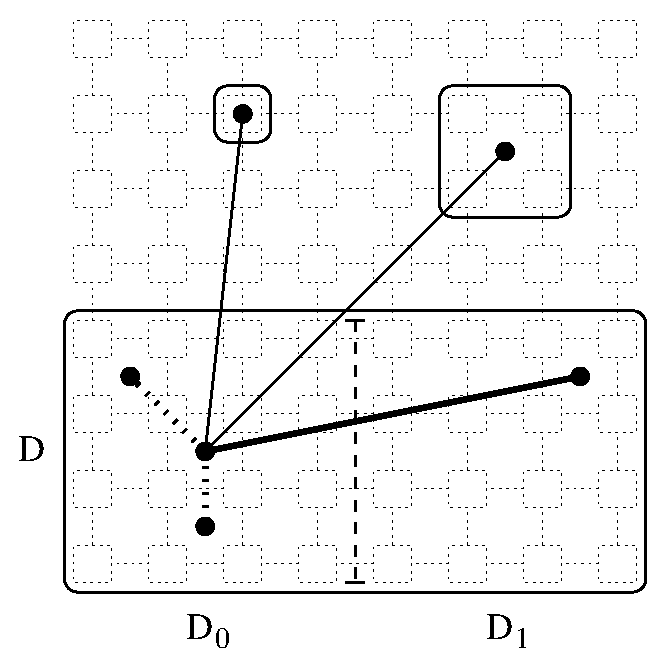
\includegraphics[scale=0.40]{s_f_rua.eps}
\hfill\\
{\bf a.} Initial position.
}\ \hfill\
\parbox[b]{4.9cm}{
\hfill
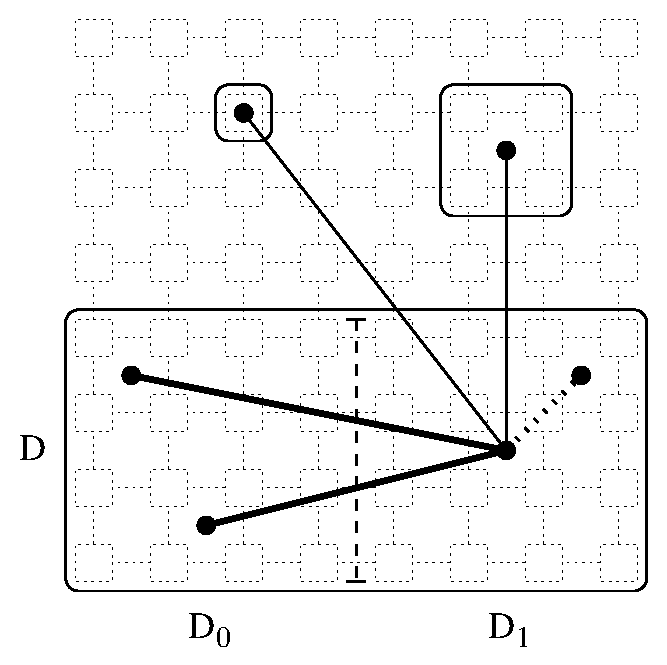
\includegraphics[scale=0.40]{s_f_rub.eps}
\hfill\\
{\bf b.} After one vertex is moved.
}\hfill\
\caption%
{Edges accounted for in the partial communication cost function when
 bipartitioning the subgraph associated with domain~$D$ between
 the two subdomains $D_0$ and $D_1$ of~$D$.
 Dotted edges are of dilation zero, their two ends being mapped onto the
 same subdomain. Thin edges are cocycle edges.}
\label{fig-bipcost}
\end{figure}

%% \subsubsection{Execution scheme}

%% From an algorithmic point of view, our mapper behaves as a greedy algorithm,
%% since the mapping of a process to a subdomain is never reconsidered, and
%% at each step of which iterative algorithms can be applied.
%% The double recursive call performed at each step induces a recursion scheme
%% in the shape of a binary tree, each vertex of which corresponds to a
%% bipartitioning job, that is, the bipartitioning of both a domain and
%% its associated subgraph.

%% In the case of depth-first sequencing, as written in the above sketch,
%% bipartitioning jobs run in the left branches of the tree have no information
%% on the distance between the vertices they handle and neighbor vertices to be
%% processed in the right branches.
%% On the contrary, sequencing the jobs according to a by-level (breadth-first)
%% travel of the tree allows any bipartitioning job of a given level to
%% have information on the subdomains to which all the processes have been
%% assigned at the previous level.
%% Thus, when deciding in which subdomain to put a given process, a
%% bipartitioning job can account for the communication costs induced by
%% its neighbor processes, whether they are handled by the job itself or not,
%% since it can estimate in $f'_C$ the dilation of the corresponding edges.
%% This results in an interesting feedback effect: once an edge has been kept
%% in a cut between two subdomains, the distance between its end vertices will
%% be accounted for in the partial communication cost function to be minimized,
%% and following jobs will be more likely to keep these vertices close to
%% each other, as illustrated in Figure~\ref{fig-biprub}.
%% \begin{figure}[hbt]
%% \hfill
%% \parbox[b]{5.2cm}{
%% \hfill
%% 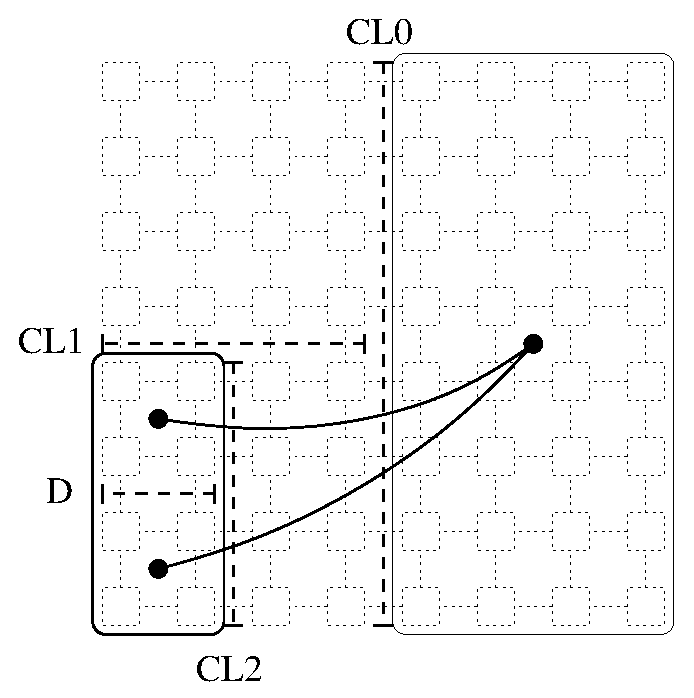
\includegraphics[scale=0.40]{s_f_run.eps}
%% \hfill\\
%% {\bf a.} Depth-first sequencing.
%% }\ \hfill\
%% \parbox[b]{5.2cm}{
%% \hfill
%% 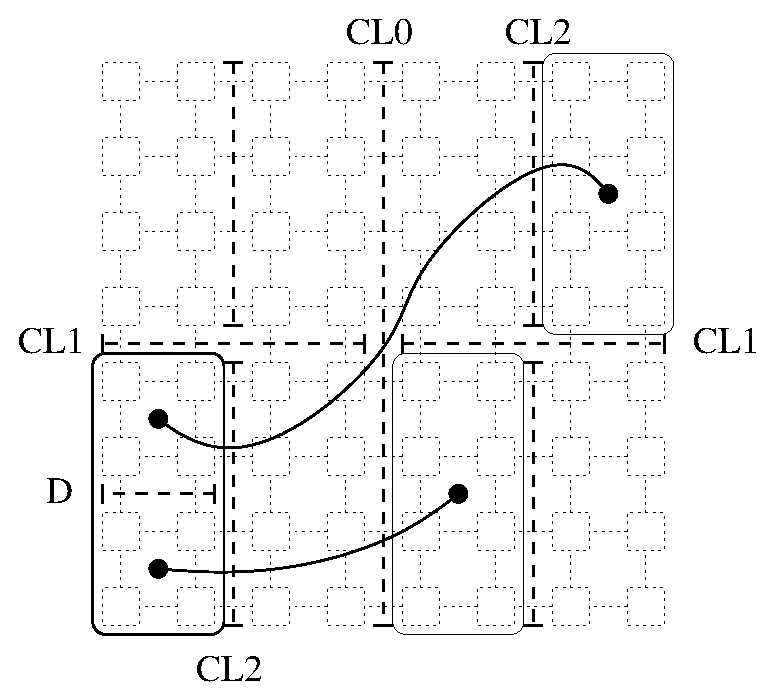
\includegraphics[scale=0.40]{s_f_ruy.eps}
%% \hfill\\
%% {\bf b.} Breadth-first sequencing.
%% }\hfill\ %
%% \caption%
%% {Influence of depth-first and breadth-first sequencings on the
%%  bipartitioning of a domain~$D$ belonging to the leftmost branch of
%%  the bipartitioning tree.
%%  With breadth-first sequencing, the partial mapping data regarding vertices
%%  belonging to the right branches of the bipartitioning tree are more
%%  accurate (C.L. stands for ``Cut Level'').}
%% \label{fig-biprub}
%% \end{figure}
%% The relative efficiency of depth-first and breadth-first sequencing schemes
%% with respect to the structure of the source and target graphs is discussed
%% in~\cite{pero96b}.

\subsubsection{Parallel graph bipartitioning methods}
\label{sec-algo-bipart}

The core of our parallel recursive mapping algorithm uses process
graph parallel bipartitioning
methods as black boxes. It allows the mapper to run any type of graph
bipartitioning method compatible with our criteria for quality.
Bipartitioning jobs maintain an internal image of the current bipartition,
indicating for every vertex of the job whether it is currently assigned to the
first or to the second subdomain.
It is therefore possible to apply several different methods in sequence,
each one starting from the result of the previous one,
and to select the methods with respect to the job characteristics, thus
enabling us to define mapping strategies.
The currently implemented graph bipartitioning methods are listed below.
\begin{itemize}
\iteme[{\bf Band}]
Like the multi-level method which will be described below, the band
method is a meta-algorithm, in the sense that it does not itself
compute partitions, but rather helps other partitioning algorithms
perform better. It is a refinement algorithm which, from a given
initial partition, extracts a band graph of given width (which only
contains graph vertices that are at most at this distance from the
separator), calls a partitioning strategy on this band graph, and
prolongs\footnote{While a \emph{projection} is an application to a
space of lower dimension, a \emph{prolongation} refers to an
application to a space of higher dimension. Yet, the term projection
is also commonly used to refer to such a propagation, most often in
the context of a multilevel framework.} back the refined partition
on the original graph. This method was designed to be able to use
expensive partitioning heuristics, such as genetic algorithms, on
large graphs, as it dramatically reduces the problem space by several
orders of magnitude. However, it was found that, in a multi-level
context, it also improves partition quality, by coercing partitions in
a problem space that derives from the one which was globally defined
at the coarsest level, thus preventing local optimization refinement
algorithms to be trapped in local optima of the finer
graphs~\cite{chpe06a}.
\iteme[{\bf Diffusion}]
This global optimization method, the sequential formulation of which
is presented in~\cite{pell07b}, flows two kinds of antagonistic
liquids, scotch and anti-scotch, from two source vertices, and sets
the new frontier as the limit between vertices which contain scotch
and the ones which contain anti-scotch. In order to add
load-balancing constraints to the algorithm, a constant amount of
liquid disappears from every vertex per unit of time, so that no
domain can spread across more than half of the vertices. Because
selecting the source vertices is essential to the obtainment of
useful results, this method has been hard-coded so that the two
source vertices are the two vertices of highest indices, since in the
band method these are the anchor vertices which represent all of the
removed vertices of each part. Therefore, this method must be used on
band graphs only, or on specifically crafted graphs.
\iteme[{\bf Multi-level}]\label{sec-algo-mle}
This algorithm, which has been studied by several
authors~\cite{basi94,hele93b,kaku95a} and should be considered as a strategy
rather than as a method since it uses other methods as parameters, repeatedly
reduces the size of the graph to bipartition by finding matchings that
collapse vertices and edges, computes a partition for the coarsest
graph obtained, and prolongs the result back to the original graph,
as shown in Figure~\ref{fig-multiproc}.
\begin{figure}[hbt]
~\hfill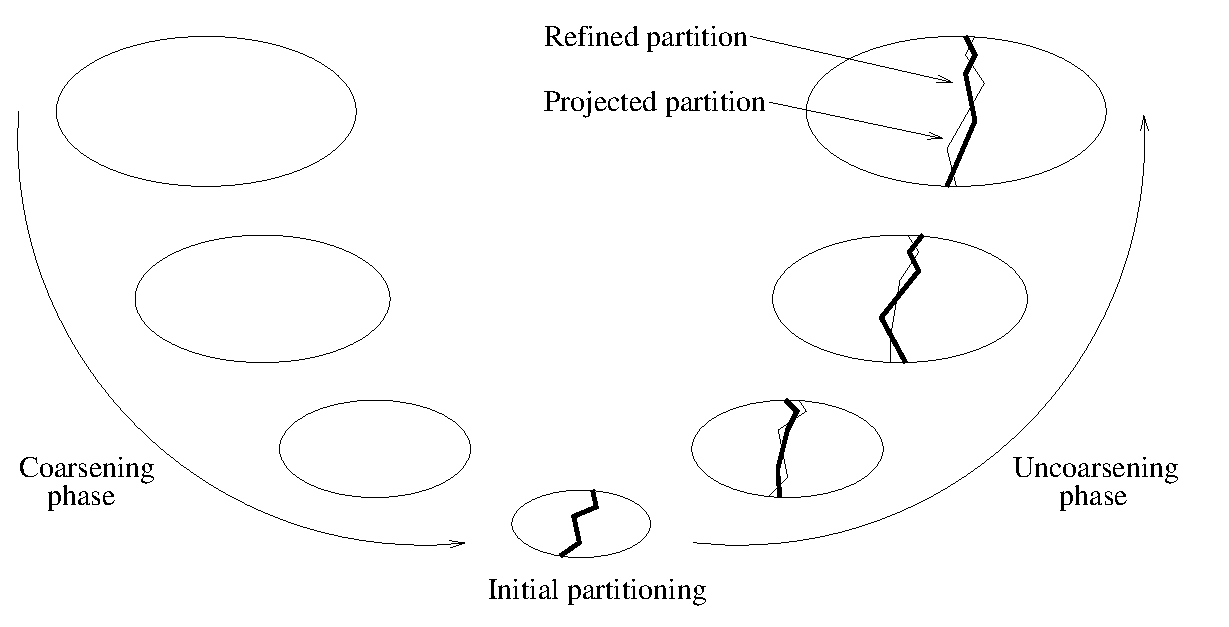
\includegraphics[scale=0.50]{s_f_mult.eps}\hfill\ ~
\caption%
{The multi-level partitioning process. In the uncoarsening phase, the light
and bold lines represent for each level the prolonged partition obtained
from the coarser graph, and the partition obtained after refinement,
respectively.}
\label{fig-multiproc}
\end{figure}
The multi-level method, when used in conjunction with the banded
diffusion method to refine the prolonged partitions at every level,
usually stabilizes quality irrespective of the number of processors
which run the parallel static mapper.
\end{itemize}

\subsubsection{Mapping onto variable-sized architectures}
\label{sec-algo-variable}

Several constrained graph partitioning problems can be modeled as
mapping the problem graph onto a target architecture, the number of
vertices and topology of which depend dynamically on the structure of
the subgraphs to bipartition at each step.

Variable-sized architectures are supported by the DRB algorithm in the
following way: at the end of each bipartitioning step, if any of the
variable subdomains is empty (that is, all vertices of the subgraph
are mapped only to one of the subdomains), then the DRB process stops
for both subdomains, and all of the vertices are assigned to their
parent subdomain; else, if a variable subdomain has only one vertex
mapped onto it, the DRB process stops for this subdomain, and the
vertex is assigned to it.

The moment when to stop the DRB process for a specific subgraph can be
controlled by defining a bipartitioning strategy that tests for the
validity of a criterion at each bipartitioning step, and maps all of
the subgraph vertices to one of the subdomains when it becomes false.

\subsection{Parallel sparse matrix ordering by hybrid incomplete nested dissection}

When solving large sparse linear systems of the form $Ax=b$, it is
common to precede the numerical factorization by a symmetric
reordering. This reordering is chosen in such a way that pivoting down
the diagonal in order on the resulting permuted matrix $PAP^T$
produces much less fill-in and work than computing the factors of $A$
by pivoting down the diagonal in the original order (the fill-in is
the set of zero entries in $A$ that become non-zero in the factored
matrix).

\subsubsection{Hybrid incomplete nested dissection}
\label{sec-algo-nested}

The minimum degree and nested dissection algorithms are the two most
popular reordering schemes used to reduce fill-in and operation count
when factoring and solving sparse matrices.
\\

The minimum degree algorithm~\cite{tiwa67} is a local heuristic that
performs its pivot selection by iteratively selecting from the graph a
node of minimum degree. It is known to be a very fast and general
purpose algorithm, and has received much attention over the last three
decades (see for example~\cite{amdadu96,geli89,liu-85}). However, the
algorithm is intrinsically sequential, and very little can be
theoretically proved about its efficiency.
\\

The nested dissection algorithm~\cite{geli81} is a global, recursive
heuristic algorithm which computes a vertex set~$S$ that separates the
graph into two parts~$A$ and~$B$, ordering $S$ with the highest
remaining indices. It then proceeds recursively on parts~$A$ and~$B$
until their sizes become smaller than some threshold value. This
ordering guarantees that, at each step, no non zero term can appear
in the factorization process between unknowns of~$A$ and unknowns
of~$B$.

Many theoretical results have been obtained on nested dissection
ordering~\cite{chro89,lirota79}, and its divide and conquer nature
makes it easily parallelizable. The main issue of the nested
dissection ordering algorithm is thus to find small vertex separators
that balance the remaining subgraphs as evenly as possible.
Provided that good vertex separators are found, the nested dissection
algorithm produces orderings which, both in terms of fill-in and
operation count, compare favorably~\cite{gukaku96,kaku95a,pero97a} to
the ones obtained with the minimum degree algorithm~\cite{liu-85}.
Moreover, the elimination trees induced by nested dissection are
broader, shorter, and better balanced, and therefore
exhibit much more concurrency in the context of parallel Cholesky
factorization~\cite[and included
references]{aseilish91,geng89,geheling88,gukaku96,pero97a,shre92}.
\\

Due to their complementary nature, several schemes have been proposed
to hybridize the two methods~\cite{hero98,kaku98a,pero97a}.
Our implementation is based on a tight coupling of the nested dissection
and minimum degree algorithms, that allows each of them to take
advantage of the information computed by the other~\cite{peroam00a}.

However, because we do not provide a parallel implementation of the
minimum degree algorithm, this hybridization scheme can only take
place after enough steps of parallel nested dissection have been
performed, such that the subgraphs to be ordered by minimum degree
are centralized on individual processors.

\subsubsection{Parallel ordering}
\label{sec-algo-parallel}

The parallel computation of orderings in \ptscotch\ involves three
different levels of concurrency, corresponding to three key steps of
the nested dissection process: the nested dissection algorithm itself,
the multi-level coarsening algorithm used to compute separators at
each step of the nested dissection process, and the refinement of the
obtained separators. Each of these steps is described below.

\paragraph{Nested dissection}

As said above, the first level of concurrency relates to the
parallelization of the nested dissection method itself, which is
straightforward thanks to the intrinsically concurrent nature of the
algorithm. Starting from the initial graph, arbitrarily distributed
across $p$ processors but preferably balanced in terms of vertices,
the algorithm proceeds as illustrated in Figure~\ref{fig-nedi}~: once
a separator has been computed in parallel, by means of a method described
below, each of the $p$ processors participates in the building of the
distributed induced subgraph corresponding to the first separated part
(even if some processors do not have any vertex of it). This induced
subgraph is then folded onto the first $\lceil\frac{p}{2}\rceil$
processors, such that the average number of vertices per processor,
which guarantees efficiency as it allows the shadowing of
communications by a subsequent amount of computation, remains
constant. During the folding process, vertices and adjacency lists
owned by the $\lfloor\frac{p}{2}\rfloor$ sender processors are
redistributed to the $\lceil\frac{p}{2}\rceil$ receiver processors so
as to evenly balance their loads.

The same procedure is used to build, on the
$\lfloor\frac{p}{2}\rfloor$ remaining processors, the folded induced
subgraph corresponding to the second part. These two constructions
being completely independent, the computations of the two induced
subgraphs and their folding can be performed in parallel, thanks to the
temporary creation of an extra thread per processor. When the vertices
of the separated graph are evenly distributed across the processors,
this feature favors load balancing in the subgraph building phase,
because processors which do not have many vertices of one part will
have the rest of their vertices in the other part, thus yielding the
same overall workload to create both graphs in the same time. This
feature can be disabled when the communication system of the target
machine is not thread-safe.

At the end of the folding process, every processor has a folded
subgraph fragment of one of the two folded subgraphs, and the nested
dissection process car recursively proceed independently on each
subgroup of $\frac{p}{2}$ (then $\frac{p}{4}$, $\frac{p}{8}$,
etc\@.) processors, until each subgroup is reduced to a single
processor. From then on, the nested dissection process will go on
sequentially on every processor, using the nested dissection routines
of the \scotch\ library, eventually ending in a coupling with minimum
degree methods~\cite{peroam00a}, as described in the previous section.

\begin{figure}
~\hfill%
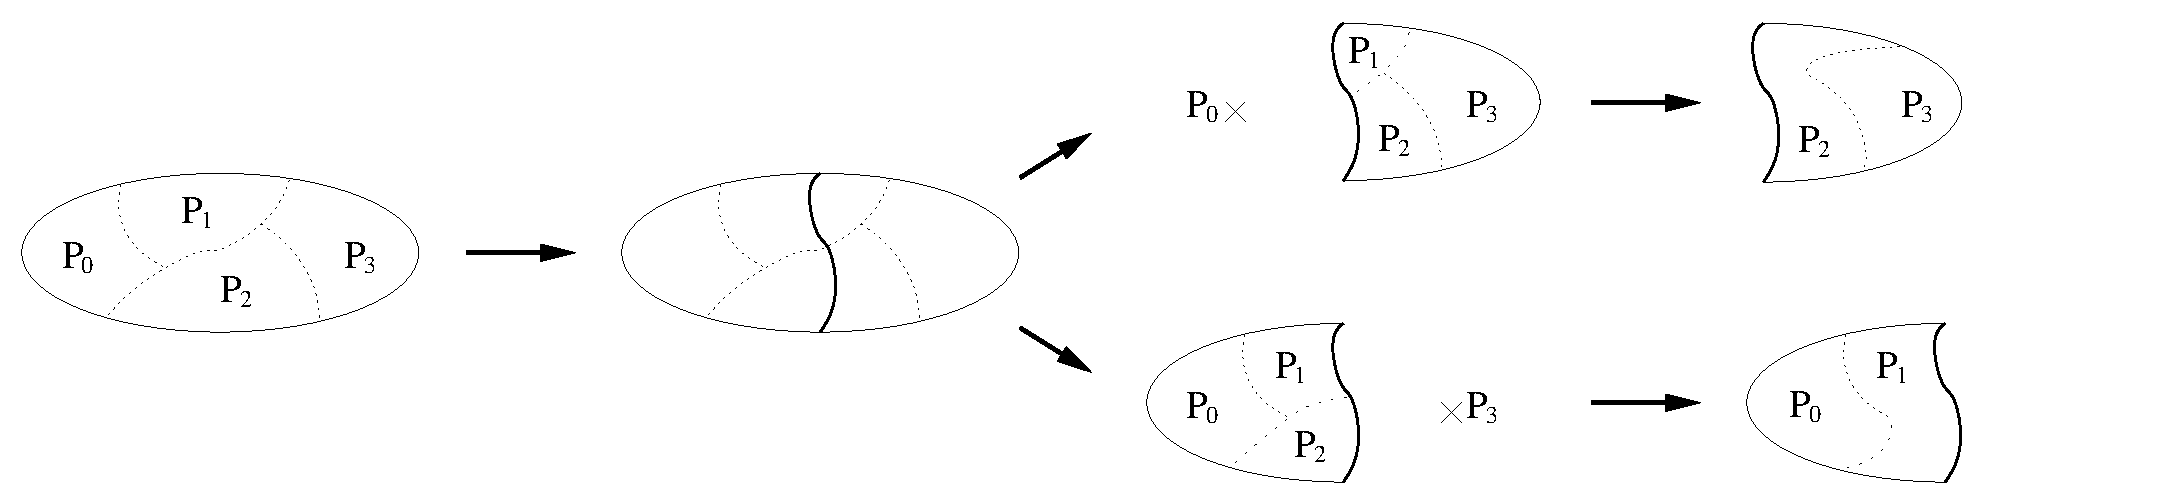
\includegraphics[scale=0.38]{p_f_nedi.eps}
\hfill~\\*[-1em]
\caption{Diagram of a nested dissection step for a (sub-)graph
  distributed across four processors. Once the separator is known, the
  two induced subgraphs are built and folded (this can be done in
  parallel for both subgraphs), yielding two subgraphs, each of them
  distributed across two processors.}
\label{fig-nedi}
\end{figure}

\paragraph{Graph coarsening}
\label{secalgocoarsen}

The second level of concurrency concerns the computation of
separators. The approach we have chosen is the now classical
multi-level one~\cite{basi94,hele95,kaku98a}. It consists in
repeatedly computing a set of increasingly coarser albeit
topologically similar versions of the
graph to separate, by finding matchings which collapse vertices and
edges, until the coarsest graph obtained is no larger than a few
hundreds of vertices, then computing a separator on this coarsest
graph, and prolonging back this separator, from coarser to finer
graphs, up to the original graph.
Most often, a local optimization algorithm, such as
Kernighan-Lin~\cite{keli70} or Fiduccia-Mattheyses~\cite{fima82} (FM), is
used in the uncoarsening phase to refine the partition that is
prolonged back at every level, such that the granularity of the
solution is the one of the original graph and not the one of the
coarsest graph.

The main features of our implementation are outlined in
Figure~\ref{fig-sepa}. Once the matching phase is complete, the
coarsened subgraph building phase takes place. It can be
parametrized so as to allow one to choose between two options. Either
all coarsened vertices are kept on their local processors (that is,
processors that hold at least one of the ends of the coarsened edges),
as shown in the first steps of Figure~\ref{fig-sepa}, which decreases
the number of vertices owned by every processor and speeds-up future
computations, or else coarsened graphs are folded and duplicated, as
shown in the next steps of Figure~\ref{fig-sepa}, which increases the
number of working copies of the graph and can thus reduce
communication and increase the final quality of the separators.

As a matter of fact, separator computation algorithms, which are local
heuristics, heavily depend on the quality of the coarsened graphs,
and we have observed with the sequential version of \scotch\ that
taking every time the best partition among two ones, obtained from
two fully independent multi-level runs, usually improved overall ordering
quality. By enabling the folding-with-duplication routine (which will
be referred to as ``fold-dup'' in the following) in the first
coarsening levels, one can implement this approach in parallel, every
subgroup of processors that hold a working copy of the graph being
able to perform an almost-complete independent multi-level
computation, save for the very first level which is shared by all
subgroups, for the second one which is shared by half of the subgroups,
and so on.

The problem with the fold-dup approach is that it consumes a lot of
memory. Consequently, a good strategy can be to resort to folding only
when the number of vertices of the graph to be considered reaches some
minimum threshold. This threshold allows one to set a trade off
between the level of completeness of the independent multi-level runs
which result from the early stages of the fold-dup process, which
impact partitioning quality, and the amount of memory to be used in
the process.

Once all working copies of the coarsened graphs are folded on
individual processors, the algorithm enters a multi-sequential phase,
illustrated at the bottom of Figure~\ref{fig-sepa}: the routines of
the sequential \scotch\ library are used on every processor to
complete the coarsening process, compute an initial partition, and
prolong it back up to the largest centralized coarsened graph stored
on the processor. Then, the partitions are prolonged back in parallel
to the finer distributed graphs, selecting the best partition between
the two available when prolonging to a level where fold-dup had been
performed. This distributed prolongation process is repeated until we
obtain a partition of the original graph.

\begin{figure}
~\hfill%
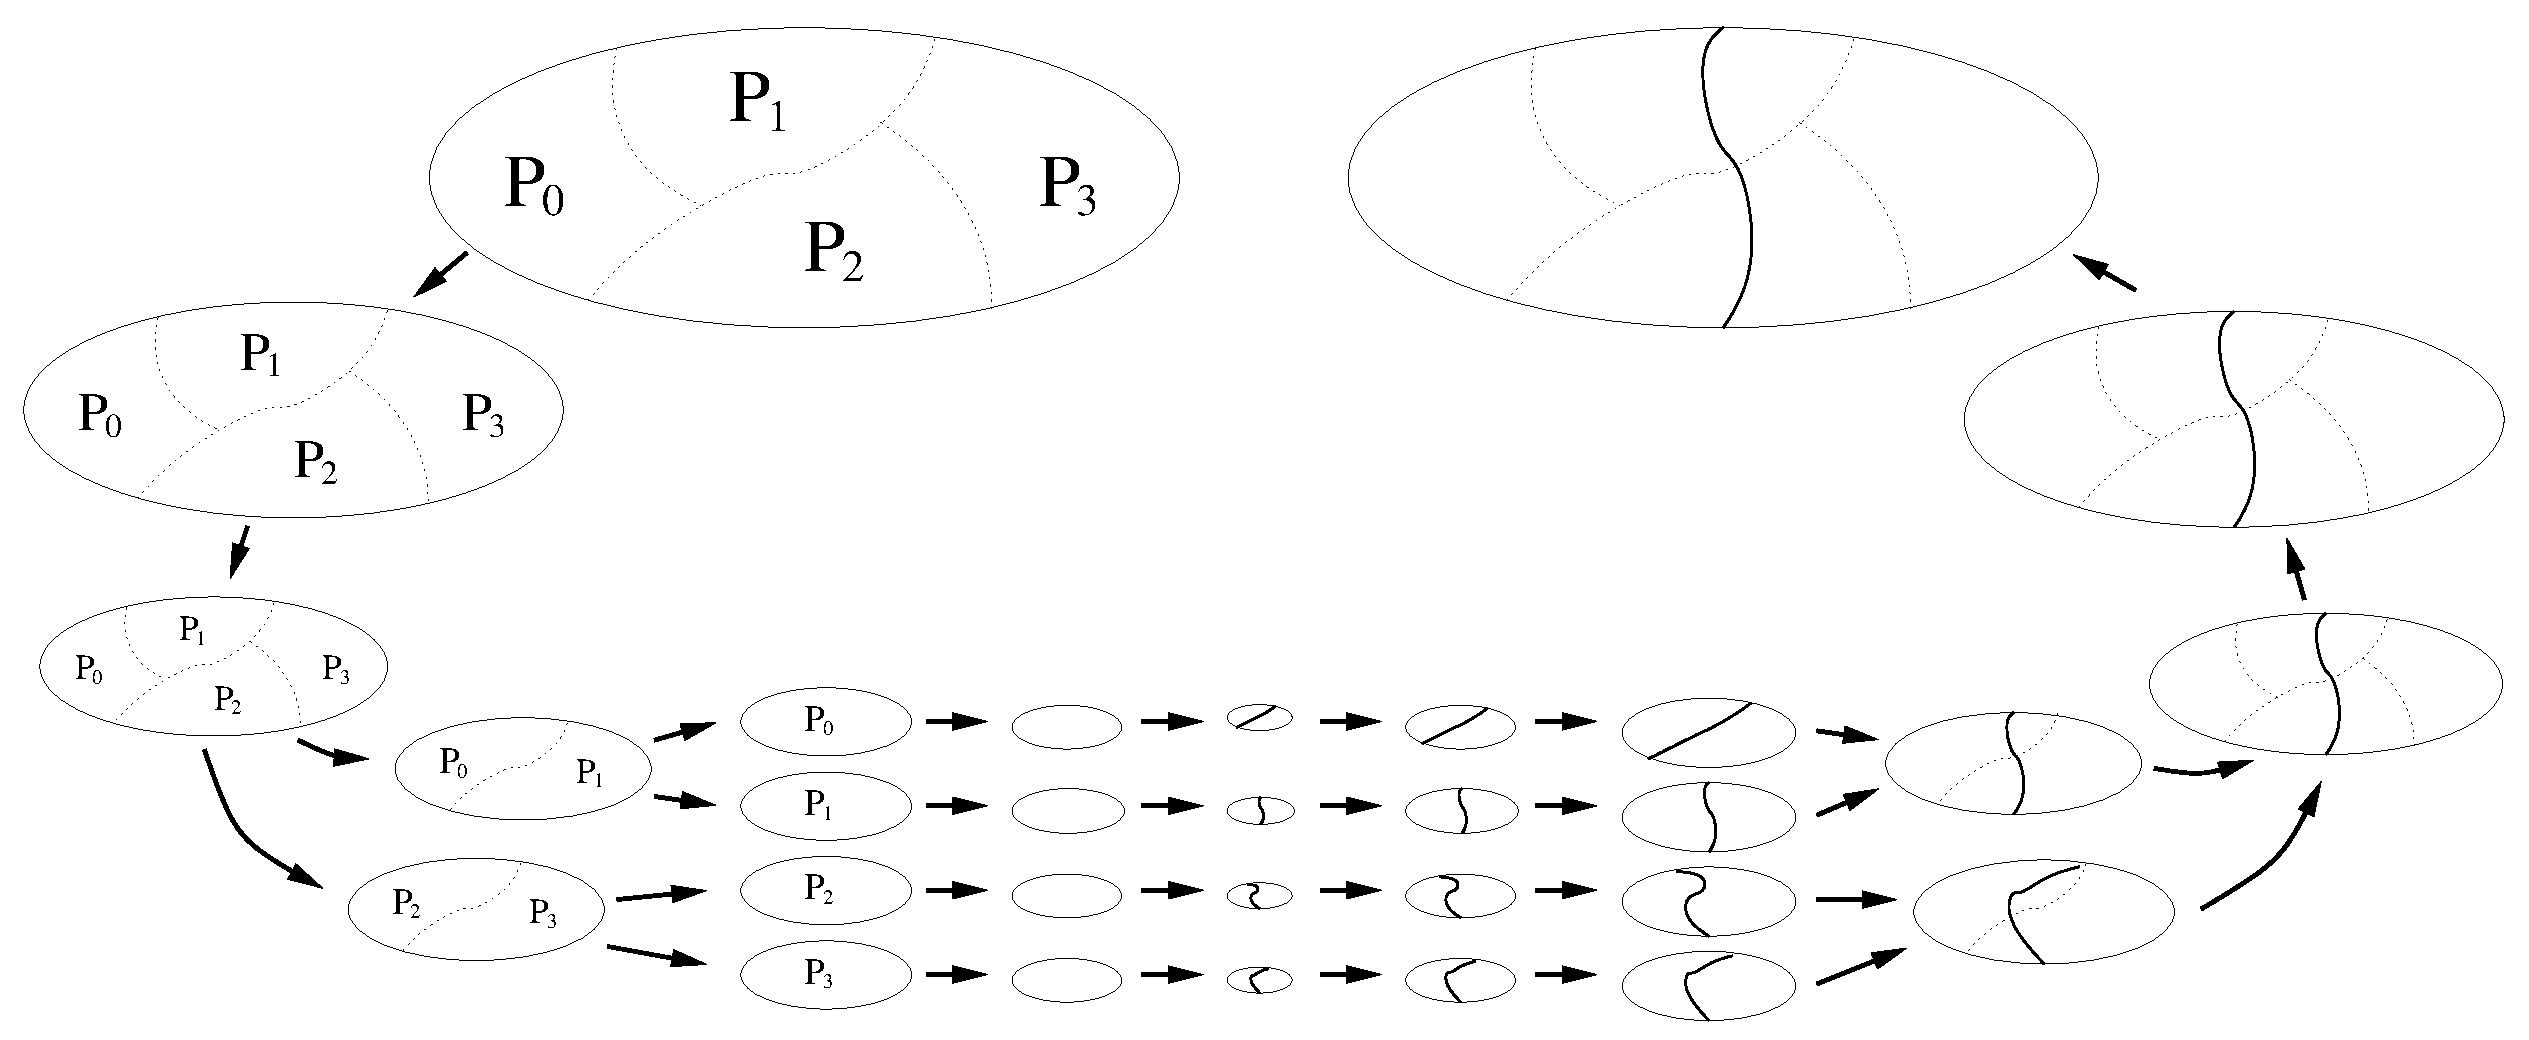
\includegraphics[scale=0.30]{p_f_sepa.eps}
\hfill~\\*[-1em]
\caption{Diagram of the parallel computation of the separator of a
  graph distributed across four processors, by parallel coarsening
  with folding-with-duplication in the last stages, multi-sequential
  computation of initial partitions that are locally prolonged back
  and refined on every processor, and then parallel uncoarsening of
  the best partition encountered.}
\label{fig-sepa}
\end{figure}

\paragraph{Band refinement}

The third level of concurrency concerns the refinement heuristics
which are used to improve the prolonged separators. At the coarsest
levels of the multi-level algorithm, when computations are restricted to
individual processors, the sequential FM algorithm of \scotch\ is
used, but this class of algorithms does not parallelize well.

This problem can be solved in two ways: either by developing
scalable and efficient local optimization algorithms, or by being able
to use the existing sequential FM algorithm on very large graphs.
In~\cite{chpe06a} has been proposed a solution
which enables both approaches, and is based on the following
reasoning. Since every refinement is performed by means of a local
algorithm, which perturbs only in a limited way the position of the
prolonged separator, local refinement algorithms need only to be
passed a subgraph that contains the vertices that are very close to
the prolonged separator.

The computation and use of distributed band graphs is outlined in
Figure~\ref{fig-band}. Given a distributed graph and an initial
separator, which can be spread across several processors, vertices
that are closer to separator vertices than some small user-defined
distance are selected by spreading distance information from all of
the separator vertices, using our halo exchange routine. Then, the
distributed band graph is created, by adding on every processor two
anchor vertices, which are connected to the last layers of vertices of
each of the parts. The vertex weight of the anchor vertices is equal
to the sum of the vertex weights of all of the vertices they replace,
to preserve the balance of the two band parts. Once the separator of
the band graph has been refined using some local optimization
algorithm, the new separator is prolonged back to the original
distributed graph.

\begin{figure}
~\hfill%
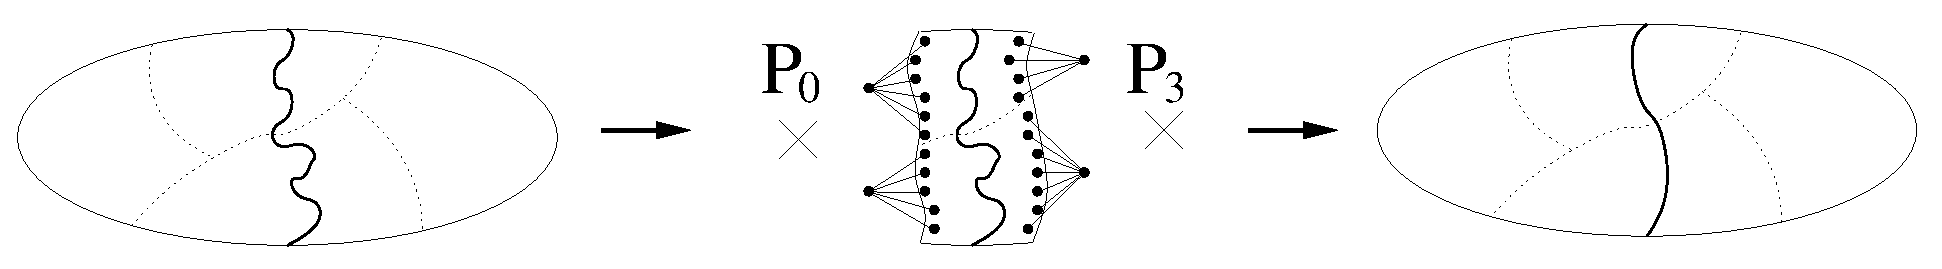
\includegraphics[scale=0.37]{p_f_band.eps}
\hfill~\\*[-1em]
\caption{Creation of a distributed band graph. Only vertices closest
  to the separator are kept. Other vertices are replaced by anchor
  vertices of equivalent total weight, linked to band vertices of the
  last layer. There are two anchor vertices per processor, to
  reduce communication. Once the separator has been refined on the
  band graph using some local optimization algorithm, the new
  separator is prolonged back to the original distributed graph.}
\label{fig-band}
\end{figure}

Basing on these band graphs, we have implemented a multi-sequential
refinement algorithm, outlined in Figure~\ref{fig-multi}. At every
distributed uncoarsening step, a distributed band graph is
created. Centralized copies of this band graph are then gathered on
every participating processor, which serve to run fully independent
instances of our sequential FM algorithm. The perturbation of the
initial state of the sequential FM algorithm on every processor allows
us to explore slightly different solution spaces, and thus to improve
refinement quality. Finally, the best refined band separator is
prolonged back to the distributed graph, and the uncoarsening process
goes on.

\begin{figure}
~\hfill%
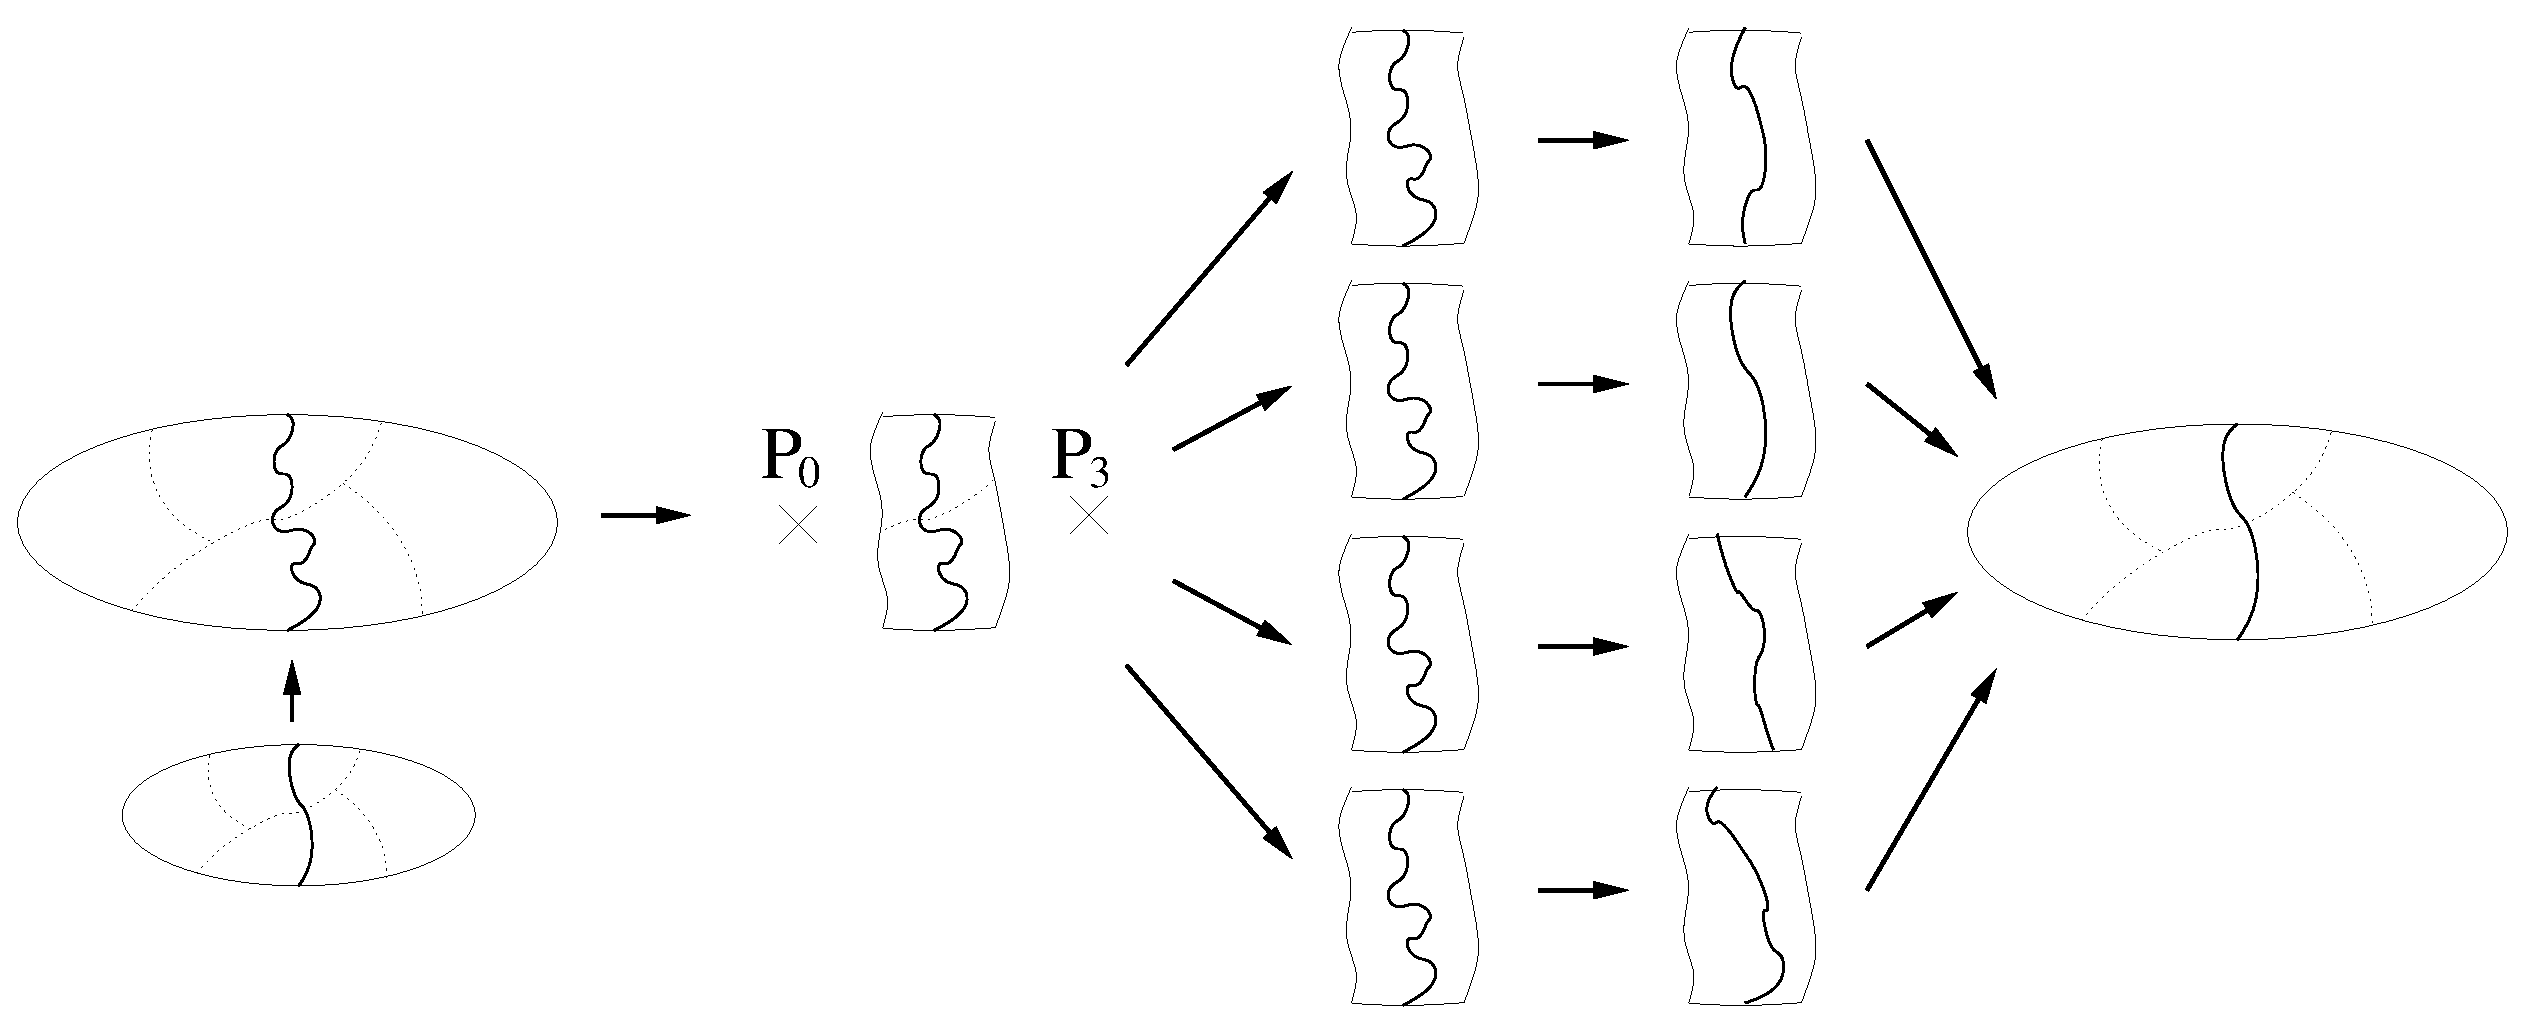
\includegraphics[scale=0.28]{p_f_multi.eps}
\hfill~\\*[-1em]
\caption{Diagram of the multi-sequential refinement of a separator
  prolonged back from a coarser graph distributed across four processors
  to its finer distributed graph. Once the distributed band graph is
  built from the finer graph, a centralized version of it is gathered
  on every participating processor. A sequential FM optimization can
  then be run independently on every copy, and the best improved
  separator is then distributed back to the finer graph.}
\label{fig-multi}
\end{figure}

\subsubsection{Performance criteria}
\label{sec-order-perf}

The quality of orderings is evaluated with respect to several
criteria. The first one, \NNZ, is the number of non-zero terms in the
factored reordered matrix. The second one, \OPC, is the operation
count, that is the number of arithmetic operations required to factor
the matrix. The operation count that we have considered takes into
consideration all operations (additions, subtractions,
multiplications, divisions) required by Cholesky factorization, except
square roots; it is equal to $\sum_c n_c^2$, where $n_c$ is the number
of non-zeros of column $c$ of the factored matrix, diagonal included.

A third criterion for quality is the shape of the elimination tree;
concurrency in parallel solving is all the higher as the elimination tree is
broad and short. To measure its quality, several parameters can be defined:
\hmin, \hmax, and \havg\ denote the minimum, maximum, and average heights
of the tree\footnote%
{We do not consider as leaves the disconnected vertices that are present in
some meshes, since they do not participate in the solving process.},
respectively, and \hdlt\ is the variance, expressed as a percentage of \havg.
Since small separators result in small chains in the elimination tree,
\havg\ should also indirectly reflect the quality of separators.
